%
Im Folgenden wird eine Betrachtung der Komplexität des in Abschnitt~\ref{sec:model_developement} entwickelten Modells präsentiert. Diese Betrachtung ist wichtig für die Parametrisierung des Optimierungsverfahrens sowie für eine Beurteilung der Generellen Lösbarkeit mit den verwendeten Verfahren. Es wird eine Visualisierung des Fitness-Raums vorgestellt und im Vergleich mit sog. Benchmark-Funktionen diskutiert.\\
%

Für die Erstellung der Fitness-Ebenen wurde ein Programmteil (der \textit{FitnessPlaneCalculator}) entwickelt, der ein Modell mit vorgegebenen Daten füttert und den Rückgabewert in eine Datei schreibt. Das Programm lässt sich per Eingabedatei steuern und erlaubt die Definition der Ebenen die dargestellt werden sollen. Es lassen sich immer zwei Variablen der Objektfunktion variieren und der Rest wird dabei auf feste Werte gesetzt. Das Erlaubt eine Visualisierung durch eine 2D-Heatmap (siehe folgende Plots). Aus der Visualisierung können Rückschlüsse auf die Gestalt der Fitnessebene gezogen werden.\\
%

Die Parameter wurde für diese Plots so gewählt, dass sie über den Bereich indem die richtige Lösung liegen sollte, iterieren. Da nur drei Parameter Variiert werden, wurden die übrigen vier auf passende Werte gesetzt. Diese konnten analytisch bestimmt werden und sind in Tabelle~\ref{tab:complexity1} zusammen mit den wahren Werten aufgeführt.\\

%
\begin{figure}[h!]
  \caption[Fitness Ebenen Heatmap]{Diese Grafik stellt die Fitnessebenen des Problems dar. Gezeigt ist das Problem für eine Anordnung aus vier Antennen und einem Sweep über die $x-y$-Ebene. Jeder Plot ist für einen festen Wert $z$ erstellt worden. Die $x, y$-Werte wurden über ein Intervall von $[-20,20]$ mit einem Inkrement von $0.5$ variiert, das ergibt eine für die Abschätzung der Gestalt der Fitnessebene ausreichende Datengrundlage. Die $z$-Werte der $16$-Plots stammen aus dem Intervall $[-7,8]$ mit einem Inkrement von $1$. Bereits in dieser Ansicht, ist zu erkennen, dass der Verlauf sehr Flach ist. Eine Schlucht bildet sich etwa in Nord-Süd-Richtung aus. Jeweils verzeinet ist das lokale Minima ($+$) eins Plots, sowie die Höhenlinien. Die farbliche Kodierung gibt den Fitnesswert an diesem Punkt an. Die Fitnesswerte wurden normiert und um den Wert ihres Minimums verschoben.}
  \begin{center}
    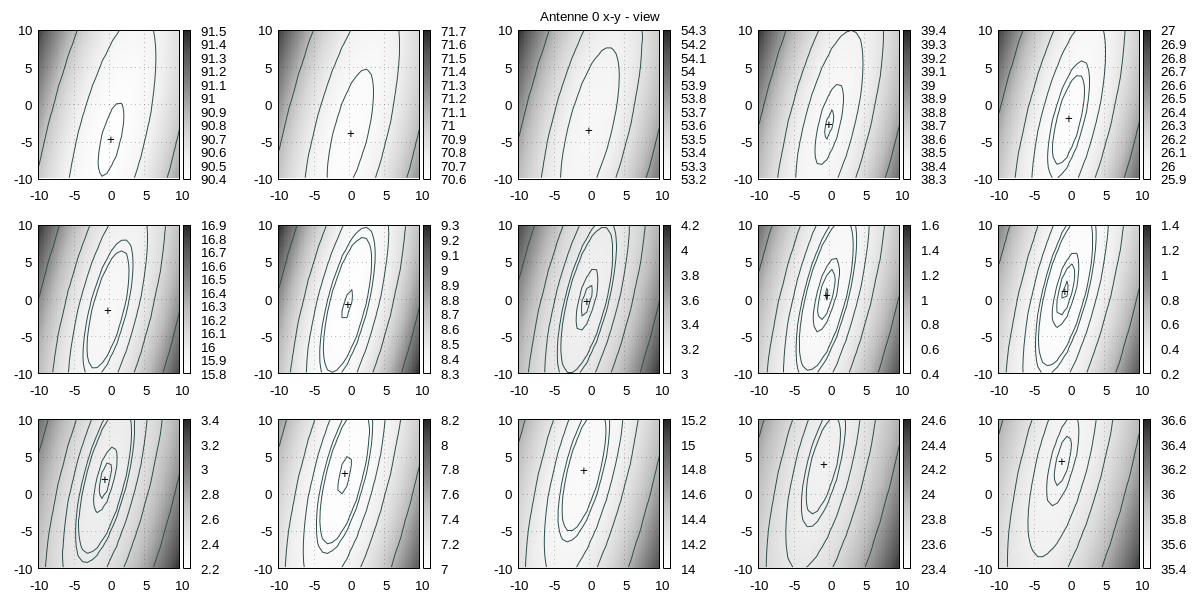
\includegraphics[width=\textwidth]{img/fitness/xy_a0.png}
  \end{center}
  \label{fig:fitnessplane1-x-y-1}
%
\end{figure}

\begin{figure}[ht!]
  \caption[Fitness Ebenen Heatmap, vergrößert]{Vergrößerung der Fitnessebenen der Antenne 1. Es ist hier deutlich zu erkennen, wie gering die Funktionen ansteigen. Das ist ein Problem für die meisten Algorithmen. Es bleibt zu klären wie sensitiv der Algorithmus auf diesen Umstand reagiert. Es wurde um das lokale Minima zentriert und der Bereich auf}
  \begin{center}
   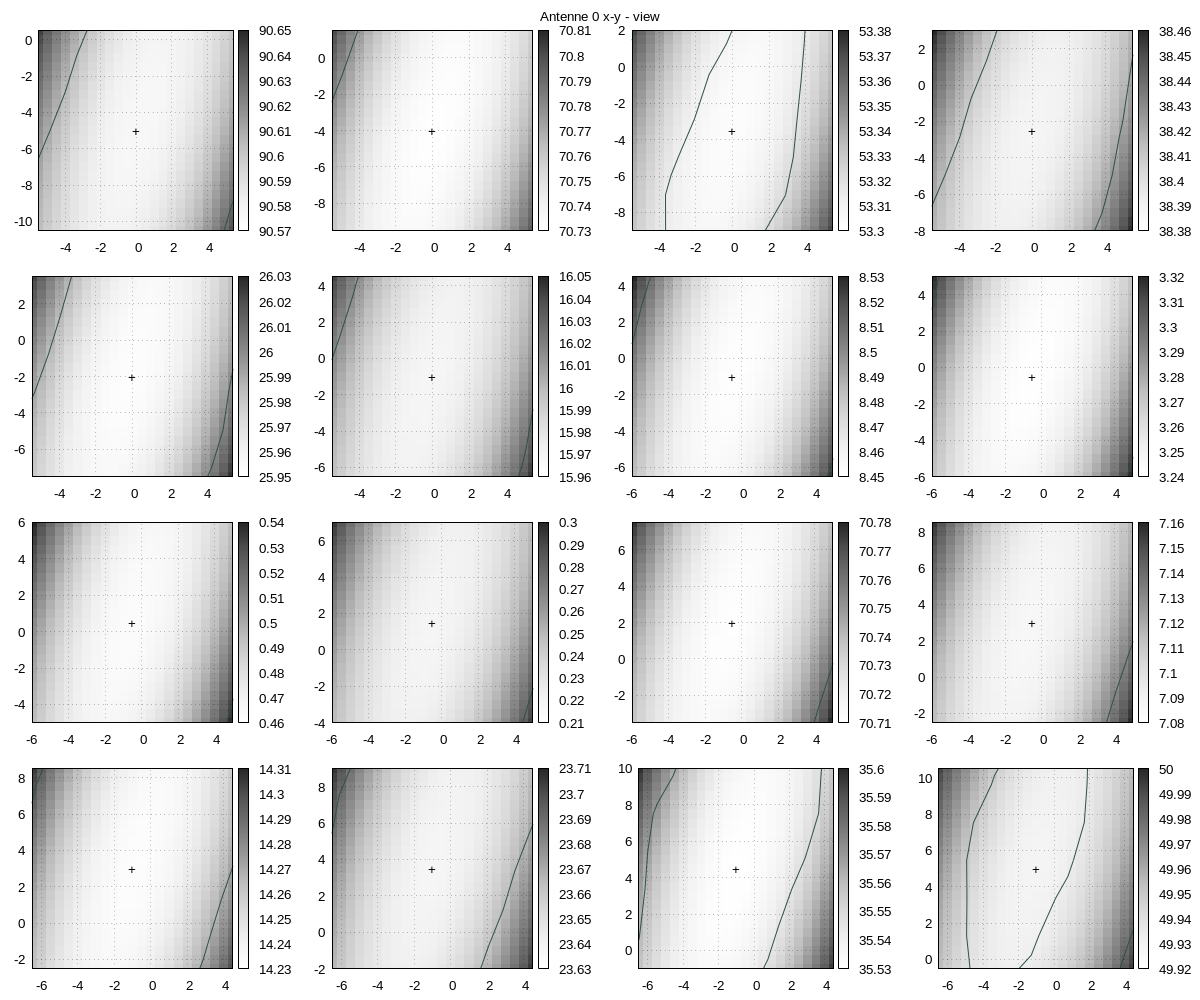
\includegraphics[width=\textwidth]{img/fitness/xy_a0zoomed.png}
  \end{center}
  \label{fig:fitnessplane1-x-y-zoom-1}
%
\end{figure}
%
In den Abbildungen~\ref{fig:fitnessplane1-x-y-1} und \ref{fig:fitnessplane1-x-y-zoom-1} zeigen sich möglicherweise die ersten Probleme für den Algorithmus. Eine große, sehr flache Fitnessebene für verschiedene Parameter ist nicht leicht zu handhaben. Aus dieser Untersuchung geht bereits hervor, dass die Anzahl an Nachkommen groß sein muss. Auch darf die Schrittweite $\sigma$ nicht zu klein werden, damit die Lösung nicht auf der flachen Ebene liegen bleibt. Ein Ähliches Verhalten zeigt sich bei den anderen Antennen und anderen Ebenen. Aufgrund der Komplexität des in dieser Arbeit erstellten Modells \ref{fig:Complexity1} ist bereits dieser Fall recht hochdimensional. Er erreicht $7$ Dimensionen und er kann im Rahmen dieser Arbeit nicht vollständig Untersucht werden. Die Fitness-Plots aller Antennen und für drei Ebenen sind in Anhang~\ref{app:fitness:plots1} zu finden. Eine vollständige Untersuchung ist indes auch nicht notwendig, da der Algorithmus den Suchraum in gewisser Weise untersucht. 
%
\begin{figure}[!h]
	 \caption[Übrige Ebenen für Antenne 1]{Auf diesen Abbildungen zeigen sich die Fitness-Ebenen für die übrigen Ansichten, x-z und y-z. In der oberen Reihe sind Ebenen über den gesamten Bereich, in der Unteren vergrößert dargestellt. Zu erkennen ist ein zum Verlauf der x-y-Ebene sehr ähnliches Bild. Ein flaches, längliches Tal mit Minimum.  }
	 \label{fig:fitnessplanesA1}
     \centering
     \begin{subfigure}[t]{0.4\textwidth}
             \centering
             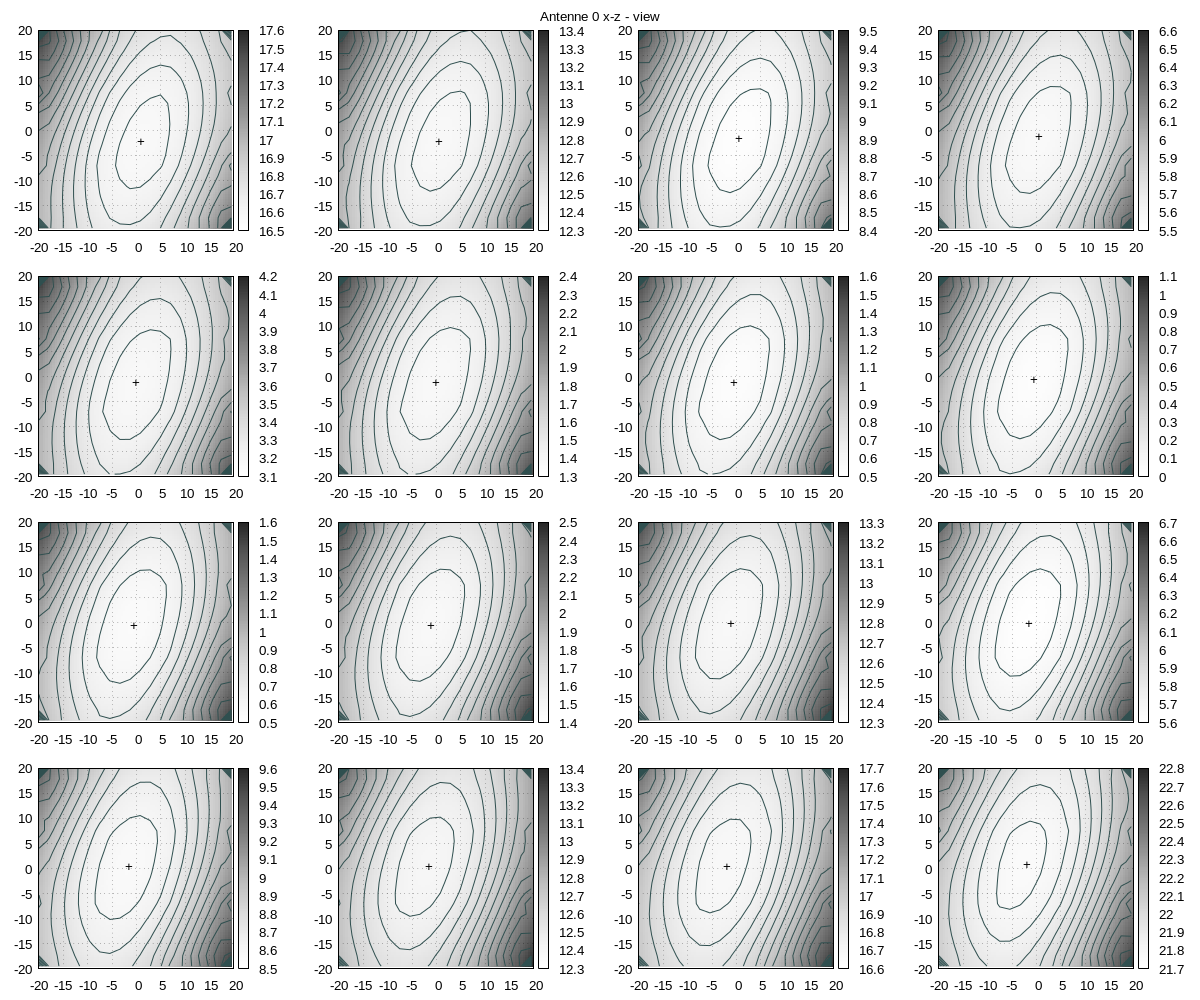
\includegraphics[width=\textwidth]{img/fitness/xz_a0.png}
%             \caption{Statistisch verteilte Endwerte für die Koordinaten der Kalibrierung.}
%             \label{fig:abortedFinal_Calibration_Ant0_ES-boxes}
     \end{subfigure}
     \qquad
     \begin{subfigure}[t]{0.4\textwidth}
			\centering
			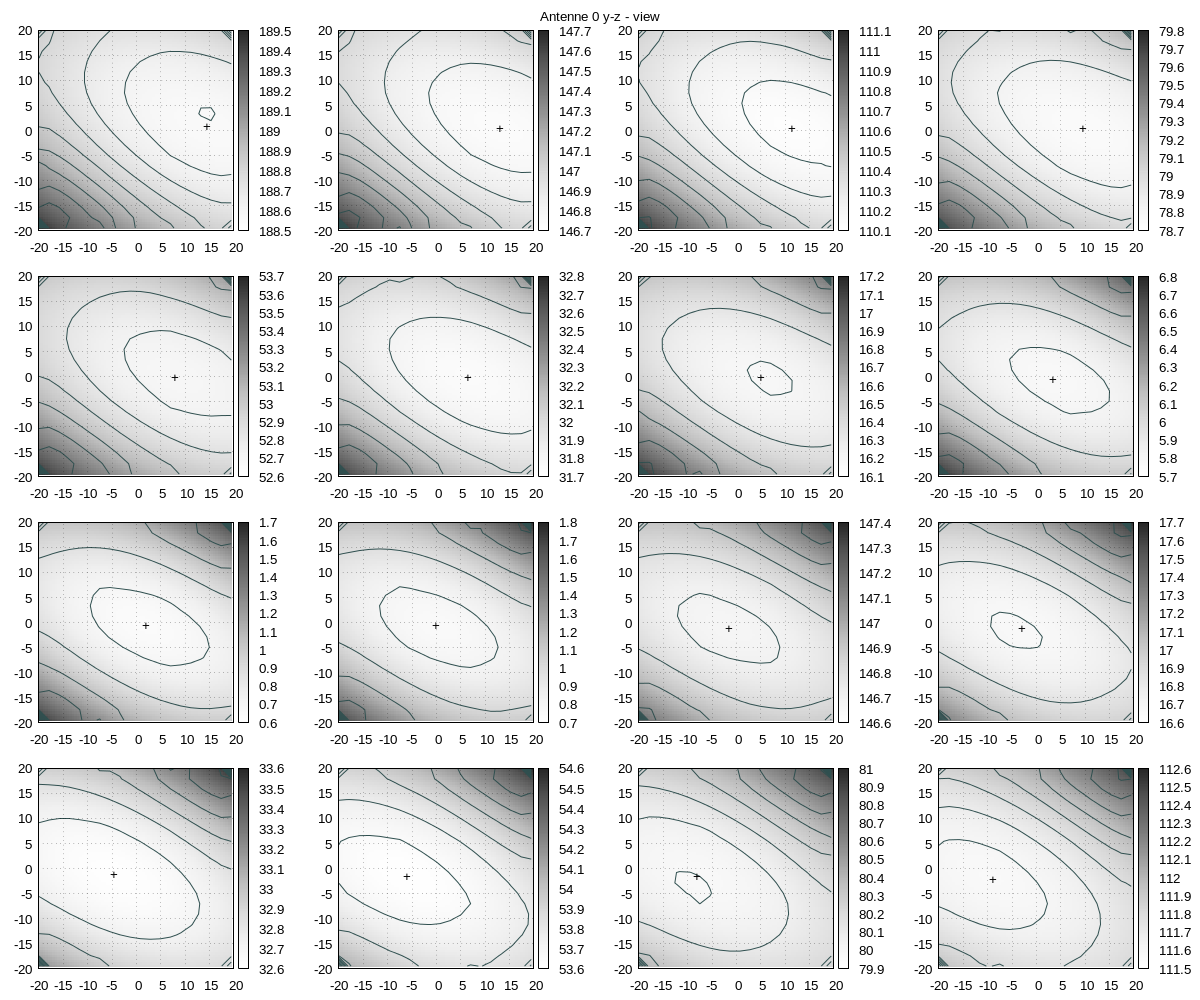
\includegraphics[width=\textwidth]{img/fitness/yz_a0.png}
%			\caption{x-z-Ebene, vergrößert}
%			\label{fig:abortedFinal_Calibration_Ant0_ES-boxes}
	 \end{subfigure}
\\
\vspace{5mm}
     \begin{subfigure}[t]{0.4\textwidth}
			\centering
			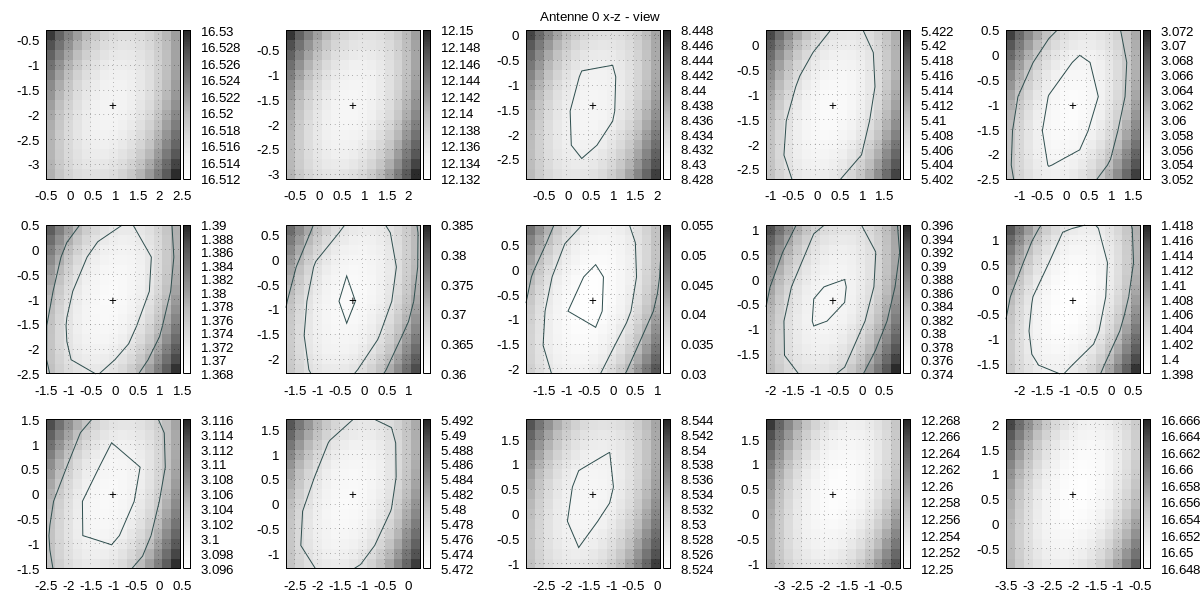
\includegraphics[width=\textwidth]{img/fitness/xz_a0zoomed.png}
%			\caption{x-z-Ebene, vergrößert}
%			\label{fig:abortedFinal_Calibration_Ant0_ES-boxes}
	 \end{subfigure}
	 \qquad
     \begin{subfigure}[t]{0.4\textwidth}
			\centering
			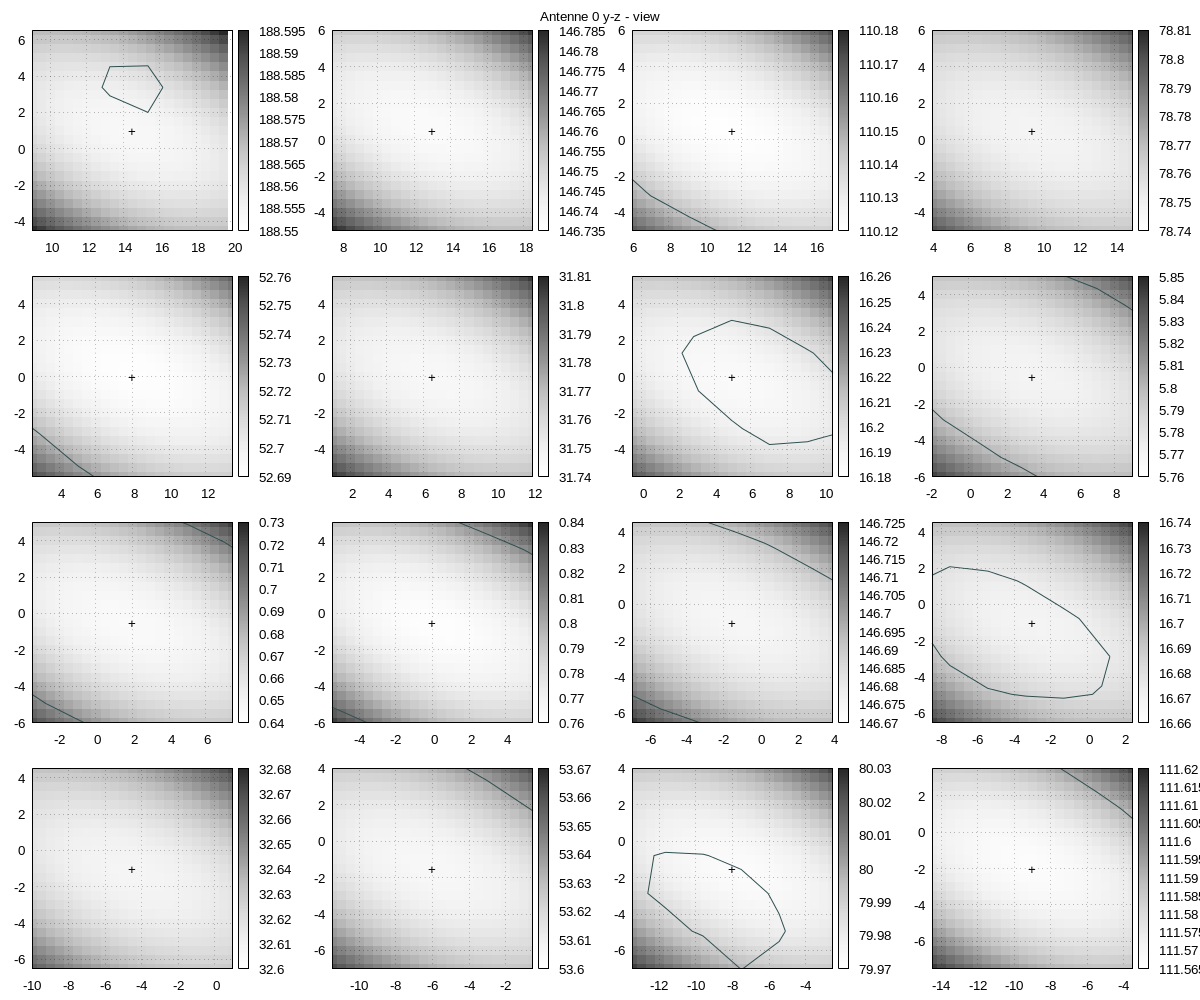
\includegraphics[width=\textwidth]{img/fitness/yz_a0zoomed.png}
%			\caption{x-z-Ebene, vergrößert}
%			\label{fig:abortedFinal_Calibration_Ant0_ES-boxes}
	 \end{subfigure}      
\end{figure}
%
\begin{table} [h]
	\begin{center}
		\begin{tabular}{lccccccc}
		\textbf{Ebene} & \textbf{$x$} & \textbf{$y$} & \textbf{$z$} & \textbf{$n_0$} & \textbf{$n_1$}& \textbf{$n_2$} & \textbf{$n_3$} \\
			\hline
			x-y & [-20:.5:20]		& [-20:.5:20]	& [-7:1:8] & [7:0:7] & [10:0:10]& [13:0:13]&[9:0:9]   \\
			x-z & [-20:.5:20] 	& [-7:1:8] 	& [-20:.5:20] & [7:0:7] & [10:0:10]& [13:0:13]&[9:0:9] \\
			y-z & [-7:1:8]  	& [-20:.5:20]	& [-20:.5:20] & [7:0:7] & [10:0:10]& [13:0:13]&[9:0:9]\\
			\hline
			Wahre & 0.479 & -1.012 & 0.607 & 7  & 10 & 13 & 9			\\
%
		\end{tabular}
		\caption[Parameter der Fitness Ebenen]{Tabellarisch sind hier die Parameter (Intervalle) der Fitness Ebenen aufgelistet. Zusätzlich sind die Werte angegeben, in denen eine optimale Lösung liegen sollte. }
		\label{tab:complexity1}
	\end{center}
\end{table}